\chapter{Intégration des formes différentielles}
Nous allons donner dans ce paragraphe la notion d'intégrale des fonctions d'une variable complexes et les propriétés les plus importantes des fonctions analytiques, attachées à cette notion. En particulier, nous établirons l'équivalence entre les fonctions analytiques dans un domaine et les fonctions dont l'intégrale ne dépend pas du chemin d'intégration. 
\section{Chemins}
Dans cette partie, on travaillera dans le cadre des ouverts de $\R^n$, qui sera dans la suite restreint à $\C$. 

\section{Intégration des formes différentielles}
\subsection{Un exemple introductif: le travail d'une force}
En mécanique, le travail d'une force est une notion fondamentale qui
permet de relier la variation d'énergie cinétique à l'intégrale d'une quantité
simple. Supposons donné un point matériel de masse $m$, se déplaçant dans
$\mathbb{R}^2$ et soumis à un champ de force $F \colon \mathbb{R}^2 \to
\mathbb{R}^2$ présent dans tout l'espace. En notant $\gamma \colon [a,b] \to
\mathbb{R}^2$ la trajectoire du point de l'instant $a$ à l'instant $b$, le principe fondamental
de la dynamique donne :
\[
 m \ddot{\gamma}(t) = F\left(\gamma(t)\right), \quad t \in [a,b].
\]
Il est possible d'obtenir une intégrale première de cette équation différentielle en prenant le
produit scalaire avec la vitesse $\dot{\gamma}(t)$ des deux côtés de
l'égalité:
\[
m \langle\ddot{\gamma}(t),\dot{\gamma}(t)\rangle =
\langle F\left(\gamma(t)\right), \dot{\gamma}(t) \rangle.
\]
Comme:
\[
\frac{\diff \|\dot{\gamma}(t)\|^2}{\diff t}(t) = 2
\langle\ddot{\gamma}(t),\dot{\gamma}(t)\rangle
\]
on obtient par intégration des deux membres, et en supposant que la vitesse est
définie en $a$ et $b$, la relation suivante :
\begin{equation}\label{eq:travail_force}
\frac{1}{2}m \|\dot{\gamma}(b)\|^2 - \frac{1}{2}m \|\dot{\gamma}(a)\|^2 =
\int_{[a,b]} \langle F\left(\gamma(t)\right), \dot{\gamma}(t) \rangle
\diff t.
\end{equation}

On reconnaît en partie gauche la variation d'énergie cinétique entre les deux positions $\gamma(a)$
et $\gamma(b)$, et en partie de droite le travail de la force $F$ le long du chemin $\gamma$. En règle générale, le travail dépend du chemin, néanmoins il existe des cas où il n'en est rien. En mécanique, ceci se produit
lorsque le champ de force $F$ dérive d'un potentiel (ou un champ scalaire), i.e. qu'il existe une application
$U \colon \mathbb{R}^2 \to \mathbb{R}$ telle que $F = \nabla U$. On
rappelle que la notation $\nabla U$ désigne le gradient de $U$ qui est
défini par la relation :
\[
\forall x \in \mathbb{R}^2, \forall v \in \mathbb{R}^2, \, \langle \nabla
U(x),v \rangle = U^\prime(x)(v)
\]
Si l'on suppose que $F$ dérive d'un potentiel $U$, le travail de $F$ s'écrit:
\begin{align*}
\int_{[a,b]} \langle F\left(\gamma(t)\right), \dot{\gamma}(t) \rangle
\diff t&  = \int_{[a,b]} \langle \nabla U(\gamma(t)), \dot{\gamma}(t)
\rangle \diff t = \int_{[a,b]} U^\prime(\gamma(t))(\dot{\gamma}(t)) \diff t \\
& = \int_{[a,b]} \frac{\diff}{\diff t}(U \circ \gamma)(t) \diff t = U\left(\gamma(b)\right) - U\left(\gamma(a)\right).
\end{align*}
Cette dernière expression ne dépend plus que des extrémités du chemin $\gamma$. 

L'expression de la variation de l'énergie cinétique (\ref{eq:travail_force}) est un exemple d'intégration d'une forme différentielle le long d'un chemin. On remarquera que la quantité $\langle F\left(\gamma(t)\right), \dot{\gamma}(t) \rangle$ exprime une projection tangentielle de $F\left(\gamma(t)\right)$ sur la courbe $\gamma$. 
\subsection{Formes différentielles}

On souhaite intégrer une fonction à valeurs dans $\R^2$, ceci le long d'un chemin $\gamma$ de classe $C^1$. Par exemple, dans l'exemple précédent, le travail d'une force est l'intégrale de la projection de la force sur le vecteur tangent à la courbe ; cette projection ayant permis de passer d'un vecteur à un nombre réel. En raison de la linéarité sur les forces, nous avons donc construit, pour chaque $t$, une forme linéaire $\omega_{\gamma(t)}$ qui associe à chaque vecteur $v \in \R^2$ attaché au point $\gamma(t)$, le nombre réel 
\begin{equation}\label{eq:formdiff1}
\omega_{\gamma(t)}(v)=\langle v, \gamma^\prime(t) \rangle = v_1 \gamma^\prime_1(t) + v_2 \gamma^\prime_2(t)
\end{equation}
L'espace des formes linéaires sur $\R^2$ est un espace vectoriel de dimension $2$ , on peut en effet prendre comme base les formes linéaires élémentaires $\diff x,\diff y$ qui à tout vecteur $v=(v_1,v_2)$ de $\R^2$ associent la $i \ieme{}$  coordonnée: $\diff x(v) = v_1$, $\diff y(v)=v_2$. Avec cette notation, la forme différentielle définie en (\ref{eq:formdiff1}) pourra s'écrire $\omega_{\gamma(t)} = \gamma^\prime_1(t) \diff x + \gamma^\prime_2(t) \diff y.$ 





% Nous supposerons que $\gamma^\prime$ ne s'annule jamais. Soit donc, $f$ une fonction continue à valeurs dans $\R^2$ continu et définie sur $\gamma([0,1])$. On peut définir le repère de Frenet associé à un point de la courbe. Il est constitué d'un vecteur tangent unitaire $\tau(t)=\gamma^\prime(t)/\|\gamma(t)\|$ et du vecteur normal $n(t)$ de façon que $(\tau(t), n(t))$ soit une base orthonormale directe. Il est alors possible de projeter $f(\gamma(t))$ dans ce repère, et de calculer les intégrale suivantes :
%\[ \int_{[0,1]} \langle f(\gamma(t)), \tau(t) \rangle \|\gamma^\prime(t)\| \diff t, \quad \int_{[0,1]} \langle f(\gamma(t)), n(t) \rangle \|\gamma^\prime(t)\| \diff t,\]
%qui existent en raison de la continuité de $f$. 
%\end{align*}


\begin{fdefn}
Soit $U$ un ouvert de $\R^2$. On appelle forme différentielle de degré $1$, une application $\omega$ de classe $C^\infty$ (ou lisse) de $U$ dans l'espace vectoriel des formes linéaires sur $\R^2$. Une telle forme $\omega$ s'écrit 
\[\omega=\alpha \diff x + \beta \diff y,\]
où $\alpha, \beta$ sont deux applications réelles $C^\infty$ définies sur $U$.
\end{fdefn}

Une forme différentielle s'interprète comme la donnée en chaque point de $U$, d'une forme linéaire, mais de plus cette forme linéaire varie de façon lisse en fonction du point de $U$. 

\begin{fdefn}
Soit $U$ un ouvert de $\R^2$. On appelle champ de vecteurs sur $U$ une application lisse de $U$ dans $\R^2$. 
\end{fdefn}
De même que pour les formes différentielles, on peut écrire un champ de vecteurs en coordonnées $X(x) = (X_1(x), X_2(x))$ avec $X_i, i=1,2$ des applications lisses de $U$ dans $\R$. Comme exemple de champ de vecteur, citons un champ de force, un champ de vent, etc. 

Toute forme différentielle $\omega$ agit sur un champ de vecteurs $X=(X_1,X_2)$ selon la formule suivante :  
\[\omega_x(X(x))=\alpha(x) X_1(x) + \beta(x) X_2(x), \quad x \in U. \]
 
\begin{exercice}
Soit $f$ une application réelle de classe $C^\infty$ définie sur un ouvert $U \subset \R^2$. Montrer que l'expression:
\[
 \diff f = \partial_x f \diff x + \partial_y f  \diff y
\]
définit une forme différentielle de degré $1$ sur $U$.
\end{exercice}

Attention, une forme différentielle de degré $1$ n'est pas forcément la différentielle d'une fonction $f$; lorsque c'est le cas, on dira que la forme $\omega$ est \textbf{exacte}. 

Par extension, une application réelle $C^\infty$, définie sur un ouvert de $ \R^2$, est appelée forme différentielle de degré $0$.



%On définit ainsi une application de $U$ dans $\R$ appelée produit contracté de $\omega$ et de $X$ et notée $(\omega | X)$. 
\begin{fdefn}
Soit $U, V$ deux ouverts de $\R^2$. Soit $\Phi \colon U \to V$ une application lisse de $U$ dans $V$. A toute forme différentielle $\omega$ sur $V$ on associe une forme $\Phi^\ast\omega$ sur $U$ définie, pour tout $x \in U$ et tout champ de vecteurs $X$ sur $U$ par la formule:
\[
\Phi^\ast\omega_x\left(X(x)\right) = \omega_{\Phi(x)}(\Phi^\prime(x).X(x))
\]
La forme $\Phi^*\omega$ est appelée image réciproque de $\omega$ par $\Phi$.
\end{fdefn}

\begin{figure}[ht]
\begin{center} \begin{tikzpicture}[line cap=round,line join=round,>=triangle 45,x=1.0cm,y=1.0cm]
\clip(4,3) rectangle (15,10);
\draw [->, color=pblue] (6.,8.) -- (7.,9);
\draw [->] (12,7.5) -- (10,4.396694449470224);
\draw [->,decorate,decoration={snake,amplitude=.8mm,segment length=4mm,post length=5mm}] (7.5,8) -- (11.,8.);
\draw [->] (6.2,7.5) -- (9.5,4.396694449470224);
\draw [->,color=pblue] (12,8) -- (13.5,8.5);
\draw (10.5,3.8) node {{\large $\Phi^\ast \omega _x ((X(x)) =\omega_{\Phi(x)}\:(\Phi^\prime(x) \cdot X(x))$}};
\begin{scriptsize}
\draw [fill=pblue] (6.,8.) circle (2.5pt);
\draw[color=pblue] (6.,7.7) node {{\large $x$}};
\draw [fill=pblue] (12,8) circle (2.5pt);
\draw[color=pblue] (12.5,7.7) node {{\large $\Phi(x)$}};
\draw[color=pblue] (7.7,9) node {{\large $X(x)$}};
\draw[color=pblue] (13.5,9) node {{\large $\Phi^\prime(x) \cdot X(x)$}};
\draw[color=black] (9,8.5) node {{\large $\Phi$}};
\draw[color=black] (7,6) node {{\large $\Phi^\ast \omega$}};
\draw[color=black] (11.5,6) node {{\large $\omega$}};
\end{scriptsize}
\end{tikzpicture}
\caption{Image réciproque d'une forme différentielle}\label{fig:pullbackform}
\end{center}
\end{figure}

Cette définition de l'image réciproque d'une forme différentielle est en quelque sorte une formule de changement de variable. Étant donné un champ de vecteurs $X$ sur $U$ et une application différentiable $\Phi\colon U \to V$, l'application dérivée $\Phi^\prime$ agit linéairement sur le champ de vecteurs selon le schéma $x \mapsto \Phi^\prime(x) \cdot X(x)$. Soit une forme différentielle sur $V$, on souhaite définir une forme différentielle sur $U$ de telle façon que lorsqu'elle agit sur les points et les vecteurs dans leurs ouverts de définition, le résultat, étant un nombre réel, ne change pas. La seule façon d'obtenir cette propriété correspond à la construction de l'image réciproque de $\omega$ (cf. figure~\ref{fig:pullbackform}).  



\begin{exercice}
En posant $\omega = \alpha \diff x + \beta \diff y$ et $\Phi=(\Phi_1,\Phi_2)$,
exprimer la forme $\Phi^\ast\omega$ sous la forme :
\[\Phi^\ast \omega = p \diff x + q \diff y,\]
en explicitant les fonctions $p(x,y)$ et $q(x,y)$. 

\textsc{Indication} : introduire la matrice jacobienne de $\Phi$. 
\end{exercice}

%On peut procéder de même pour les champs de vecteurs, mais il s'agira ici d'une image directe.
%
%\begin{fdefn}
%Soit $U,V$ deux ouverts de $\R^2$. Soit $\Phi \colon U \to V$ un difféomorphisme $C^\infty$. A tout champ de vecteurs $X$ défini sur $U$, on associe un champ de vecteurs $\Phi_\ast X$ sur $V$ par la formule :
%\[\Phi_\ast X(x) = \Phi^\prime(y)\cdot X(y)
%\]
%avec $y = \Phi^{-1}(x)$.
%\end{fdefn}
%Contrairement à l'image réciproque d'une forme différentielle, l'image directe d'un champ de vecteurs n'est définie que pour des difféomorphismes. Il découle des définitions que les images directes et réciproques sont d'une certaine façon des opérations adjointes (cf. figure~\ref{fig:pullbackform}) pour l'accouplement de dualité $\langle \omega, v\rangle_x=\omega_x(v)$ entre les formes différentielles et les vecteurs. En effet, nous avons l'identité
%\[\langle \Phi^\ast \omega,  X \rangle_x  = \langle \omega , \Phi_* X \rangle_{\Phi(x)}.\]
%
%%La proposition suivante découle directement des définitions et montre que les images directes et réciproques sont d'une certaine façon des opérations adjointes (cf. figure~\ref{fig:pullbackform}) :  
%%\begin{prop}
%%Soit $U,V$ ouverts de $\R^2$. Soit $\Phi \colon U \to V$ un difféomorphisme $C^\infty$. Pour toute forme différentielle $\omega$ de degré 1 sur $V$ et tout champ de vecteurs $X$ sur $U$ on a :
%%\[\Phi^\ast \omega  X \right) = \left(\omega | \phi_* X \right)
%%\]
%%\end{prop}
On peut étendre la notion de forme différentielle en définissant les formes différentielles de degré $2$. 
\begin{fdefn}
Une forme différentielle de degré $2$ sur un ouvert $U \subset \R^2$ est une application $C^\infty$ de $U$ dans l'espace des formes bilinéaires alternées sur $\R^2$. Une telle forme s'écrit sous la forme
\[\omega=f \diff x \wedge \diff y,\]
où $f$ est une application $C^\infty$ sur $U$ et $\diff x \wedge \diff y$ est la forme bilinéaire alternée agissant sur les vecteurs $u, v$ de $U$ selon la formule suivante :
\[\diff x \wedge \diff y (u,v) = \det(u,v)=u_1v_2 - u_2v_1,\]
où $\det$ désigne le déterminant. 
\end{fdefn}

Rappelons que l'espace des formes bilinéaires alternées sur $\R^p$ est de dimension $p(p-1)/2$. Lorsque $p=2$, la dimension est égale à $1$ ; la forme $\diff x \wedge \diff y$ étant alors un vecteur de base. Notons également que l'action de $\diff x \wedge \diff y$ sur les vecteurs $u,v$ donne l'aire signée du parallélogramme défini par $u$ et $v$.

Une forme différentielle de degré $2$ agira donc sur deux champs de vecteurs $X, Y$, selon le mode suivant :
\[\omega_x(X,Y)=f(x)\left[X_1(x) Y_2(x) - X_2(x)Y_1(x)\right], \quad x \in U.\]

%%\begin{notation}
%L'ensemble des formes différentielles de degré $p$ et de régularité $k$ sur un ouvert $U$ de $\R^n$ sera noté $\Omega_k^p(U)$.
%%\end{notation}
%Contrairement au cas particulier $p=1$, une contrainte supplémentaire est exigée: le caractère alterné des formes linéaires. La raison de ce choix apparaîtra dans la suite lorsque on voudra interpréter une intégrale de forme comme une intégrale ordinaire.
%Toute forme $p$-linéaire alternée sur $\R^n$ avec $p > n$ est identiquement nulle, on ne considérera donc que des formes de degré au plus $n$. L'espace vectoriel des formes $p$-linéaires alternées sur $\R^n$ est de dimension $C_n^p$. En effet, par la propriété de $p$-linéarité, il est suffisant de considérer l'action sur les $p$-uplets de vecteurs de base $(e_{i_1},\dots e_{i_p})$ où les indices $i_1,\dots i_p$ sont dans l'ensemble $\{1, \dots n\}$. Le caractère alterné permet de se restreindre encore aux seuls $p$-uplets $(e_{i_1},\dots e_{i_p})$ formés d'indices distincts rangés en ordre croissant, i.e. tels que $i_1 < i_2 < \dots < i_p$. On définit alors les formes $p$-alternées de base sur de tels $p$-uplets par:
%\[
%dx^{i_1\dots i_p}(e_{j_1},\dots,e_{j_p}) = \begin{cases}
%1 \text{ si } i_1=j_1,\dots i_p=j_p \\
%0 \text{ sinon }
%\end{cases}
%\]
%\begin{fprop}
%Soit $(v_1,\dots,v_p)$ un $p$-uplets de vecteurs de $\R^n$. On a:
%\[
%dx^{i_1\dots i_p}(v_1,\dots,v_p) = det(M) 
%\]
%où $M$ est la matrice $p \times p$ dont les lignes sont formées des coordonnées d'indice $i_1, \dots, i_p$ des vecteurs $v_1,\dots v_p$.
%\end{fprop}
%\begin{proof}
%Par la $p$ linéarité et en notant $v_{jk}$ la coordonnée $k$ du vecteur $j$:
%\[
%dx^{i_1\dots i_p}(v_1,\dots,v_p) = \sum_{(k_1,\dots,k_p)} \prod_{j=1}^p v_{jk_j}dx^{i_1\dots i_p}(e_{k_1},\dots,e_{k_p})
%\]
%La définition des formes de base $dx^{i_1\dots i_p}$ montre que seuls les termes correspondant à des indices appartenant à l'ensemble $I = \{i_1, \dots , i_p\}$ sont non nuls. Il vient donc:
%\[
%dx^{i_1\dots i_p}(v_1,\dots,v_p) = \sum_{(k_1\in I,\dots,k_p\in I)} \prod_{j=1}^p v_{jk_j}dx^{i_1\dots i_p}(e_{k_1},\dots,e_{k_p})
%\]
%En utilisant le caractère alterné des formes, on peut se ramener par changement de signe au seul cas où les indices sont rangés en ordre croissant, qui donne une valeur de $1$ pour la forme de base. On en déduit l'expression:
%\[
%dx^{i_1\dots i_p}(v_1,\dots,v_p) = \sum_{\sigma \in \Sigma(I)} \epsilon(\sigma) \prod_{j=1}^p v_{j\sigma(i_j)}
%\]
%où $\Sigma(I)$ désigne l'ensemble des permutations de $I$ et $\epsilon(\sigma)$ la signature de la permutation $\sigma$. On remarque alors que cette expression est celle donnant le déterminant de la matrice $M$. 
%\end{proof}
%\begin{fdefn}
%Un $p$-uplet d'indices $I=(i_1, \dots, i_p)$ est appelé multi-indice de longueur $p$. Il est dit ordonné si $i_1 < \dots < i_p$. La longueur d'un multi-indice $I$ est notée $|I|$.
%\end{fdefn}
%%\begin{notation}
% Soit $I=(i_1, \dots, i_p)$ un multi-indice ordonné. On notera $dx^I$ la forme de base $dx^{i_1,\dots,i_p}$.
%%\end{notation}
%
%Il est possible de définir un produit entre les formes différentielles, que l'on notera $\wedge$. 
%Pour ce faire, on supposera donnés  deux multi-indices ordonnés disjoints $I=(i_1, \dots , i_p)$ et $J=(j_1, \dots j_q)$. Soit $K$ le multi-indice ordonné  $(k_1,\dots,k_{p+1})$ obtenu à partir des éléments de l'ensemble $I\cup J = \{i_1,\dots,i_p,j_1,\dots,j_q\}$. 
%Il existe une unique permutation $\sigma$ associant à $(i_1,\dots,i_p,j_1,\dots,j_q)$ le multi-indice $K$. On pose:
%\[
%dx^I \wedge dx^J = \epsilon(\sigma) dx^K
%\]
%Si les deux multi-indices ordonnés $I,J$ ne sont pas disjoints, on posera $dx^I \wedge dx^J = 0$.
%Un produit étant une application bilinéaire, $\wedge$ est défini de façon unique pour des formes quelconques à partir de la relation précédente. L'opération $\wedge$ est appelée produit extérieur. 
%\begin{fprop}
%Soient $\omega,\theta,\rho$ trois formes multilinéaires alternées de degrés respectifs $p,q,r$. On a:
%\begin{enumerate}
%\item $\omega \wedge \theta = (-1)^{pq} \theta \wedge \omega$.
%\item $(\omega \wedge \theta) \wedge \rho = \omega \wedge (\theta \wedge \rho)$.
%\item $\omega \wedge \omega = 0$.
%\end{enumerate}
%\end{fprop}
%\begin{proof}
%Il suffit de vérifier ces propriétés sur les formes de base $dx^I$, sur lesquelles elles sont immédiates.
%\end{proof}
%On notera que pour tout multi-indice ordonné $I=(i_1,\dots,i_p)$ on a $dx^I = dx_{i_1}\wedge \dots \wedge dx_{i_p}$.
%La proposition suivante est une conséquence directe du fait que les formes $dx^I$, avec $I$ multi-indice ordonné de longueur $p$, forment une base de $\Lambda_n^p$.
%\begin{fprop}
%Soit $U$ un ouvert de $\R^n$. Toute forme différentielle $\omega$ de $\Omega_k^p(U)$ s'écrit de façon unique:
%\[
%\omega \colon x \in U \mapsto \sum_I \omega_I(x) dx^I
%\]
%où la somme porte sur tous les multi-indices ordonnées de longueur $p$, avec $\omega_I \colon U  \mapsto \R$ de classe $C^k$.
%\end{fprop}
%Le produit extérieur s'étend aux formes différentielles de la façon suivante:
%\begin{fdefn}
%Soit $\omega = \sum_I \omega_I dx^I$ une forme différentielle de $\Omega_k^p$ et $\theta = \sum_J \theta_J dx^J$ une forme différentielle de $\Omega_k^q$. Le produit extérieur de $\omega$ et $\theta$, noté $\omega \wedge \theta$ est défini par:
%\[
%\omega \wedge \theta = \sum_{I\cap J = \emptyset} \omega_I \theta_J dx^I \wedge dx^J 
%\]
%\end{fdefn}
%Le produit extérieur des formes différentielles vérifie les mêmes propriétés que celui des formes multilinéaires alternées. 

%Une forme différentielle de degré $p$ agit sur les $p$-uplets de champs de vecteurs sur $U$ selon la formule:
%\[
%\left(\omega|X_1,\dots,X_p\right) \colon x \in U \mapsto \omega\left(x;X_1(x),\dots,X_p(x)\right)
%\]

Rappelons qu'en raison du caractère alterné, nous avons
\[\omega(X,Y)=-\omega(Y,X), \quad \omega(X,X)=0.\]


La définition suivante est une généralisation directe de ce qui a été vu pour les formes de degré 1. 
\begin{fdefn}
Soit $U,V$ deux ouvert de $\R^2$. Soit $\Phi \colon U \to V$ une application lisse. A toute forme différentielle $\omega$ de degré $2$ on associe la forme $\Phi^\ast \omega$ de degré $2$ sur $U$ définie, pour tout $x \in U$ et tous champs de vecteurs $X,Y$ sur $U$ par la formule :
\[\Phi^\ast\omega_x(X(x), Y(x)) = \omega_{\Phi(x)}(\Phi^\prime(x)\cdot X(x),\Phi^\prime(x)\cdot Y(x))
\]
La forme $\Phi^*\omega$ est appelée image réciproque de $\omega$ par $\Phi$.
\end{fdefn}

%De même que pour les formes de degré 1, l'image réciproque des formes différentielles et l'image directe des champs de vecteurs sont des opérations adjointes : 
%\[\langle \Phi^\ast \omega, (X,Y) \rangle_x =  \langle \omega, (\Phi_\ast X, \Phi_\ast Y) \rangle_{\Phi(x)}.\]
%\begin{prop}
%Soit $U,V$ ouverts de $\R^n$. Soit $\phi \colon V \to U$ un difféomorphisme de classe $C^{k+1}$. Pour toute forme différentielle de $\Omega_k^p$ et tout $p$-uplet $(X_1,\dots, X_p)$ de champs de vecteurs de classe $C^k$ sur $V$ on a:
%\[
%\left(\phi^* \omega | X_1,\dots X_p \right) = \left(\omega | \phi_* X_1,\dots,\phi_* X_p \right)
%\]
%\end{prop}
%Le produit extérieur commute avec l'image réciproque:
%\begin{fprop}
%Soit $U$ ouvert de $\R^m$ et $V$ ouvert de $\R^n$. Soit $\phi \colon U \to V$ une application de classe $C^{k+1}$. Pour toute forme $\omega$ de $\Omega_k^p(V)$ et $\theta$ de $\Omega_k^q(V)$ on a:
%\[
%\phi^*(\omega \wedge \theta) = (\phi^*\omega)\wedge(\phi^*\theta)
%\]
%\end{fprop}
%\begin{proof}
%Il suffit de le vérifier sur des formes constantes $dx^I$,$dx^J$ respectivement éléments de $\Omega_k^p(V)$ et $\Omega_k^q(V)$. Soient $v_1,\dots,v_{p+q}$ des vecteurs de $\R^m$. On a, en posant comme précédemment $K$ le multi-indice ordonné obtenu à partir de $I\cup J$ et $\sigma$ la permutation ramenant $(i_1,\dots,i_p,j_1,\dots j_q)$ sur $K$:
%\begin{align*}
%\phi^*(dx^I \wedge dx^J)(x;v_1,\dots,v_{p+q}) & = \epsilon(\sigma) dx^K(x;\phi^\prime(x).v_1,\dots,\phi^\prime(x).v_{p+q}) \\
%&  = (\phi^*dx^I)\wedge(\phi^*dx^J)(x;v_1,\dots,v_{p+q})
%\end{align*}
%\end{proof}
%Cette proposition est très importante pour le calcul: comme toute forme de base $d^{i_1,\dots,i_p}$ peut s'écrire $dx_{i_1} \wedge \dots \wedge dx_{i_p}$, il suffit de déterminer l'image réciproque des formes de base de degré 1 pour pouvoir l'obtenir sur des formes quelconques. 


\begin{exercice}
Pour cet exercice, on se place dans l'ouvert $V = \R^2-\{(0,0)\}$. Soit la forme différentielle $\omega = \diff x \wedge \diff y$.
\begin{enumerate}
\item Montrer que l'application $\Phi \colon (\rho,\theta) \mapsto (\rho \cos \theta, \rho \sin \theta )$ de $\R^{+*}\times [0,2\pi]$ dans $V$ est de classe $C^\infty$. Est-ce un difféomorphisme ?
\item Déterminer l'image réciproque de $\omega$ par $\Phi$. 
\end{enumerate}

\textsc{Indication}: On déterminera la matrice jacobienne de $\Phi$ que l'on appliquera à $(X_\rho, X_\theta)$. On peut aussi utiliser le fait que l'aire signée du parallélogramme, défini par l'image de deux vecteurs par une application linéaire, est égale à l'aire du parallélogramme, défini par les deux vecteurs, multipliée par le déterminant de la matrice de l'application linéaire.
\end{exercice}

%Soit $f \colon U \to \R$ de classe $C^k$ que l'on considérera comme forme de degré 0. Pour tout point $x$ de $U$, $f^\prime(x)$ est une forme linéaire sur $\R$ qui a $v$ associe le scalaire:
%\[
%f^\prime(x).v = \sum_{i=1}^n \frac{\partial f}{\partial x_i} v_i 
%\]
%elle s'identifie donc avec la forme $df = \sum_{i=1}^n \frac{\partial f}{\partial x_i} dx_i$, déjà vue en exercice. 
%Soit maintenant $\omega$ une forme différentielle de $\Omega_k^p(U)$ avec $U$ ouvert de $\R^n$ et $p \geq 1$. Pour un point $x$ de $U$ donné, $\omega^\prime(x)$ est une application linéaire de $\R^n$ dans $\Lambda_n^p$, que l'on peut aussi voir comme une application multilinéaire qui a un $p+1$-uplet de vecteurs $v_1, \dots, v_{p+1}$ associe $\omega^\prime(x)(v_1)(v_2,\dots,v_{p+1})$. Cette application n'est pas alternée: le premier vecteur $v_1$ est l'argument sur lequel s'applique la dérivée en $x$ et sa permutation avec l'un des $v_i, i > 1$ n'a pas de propriété particulière. Contrairement à ce qui se passe pour les formes de degré 0, la dérivée usuelle d'une forme différentielle n'est pas une forme différentielle. Pour remédier à ce problème et obtenir une véritable dérivation, une démarche constructive va être suivie. On notera $d$ la dérivation que l'on va progressivement définir. La première hypothèse qui doit être satisfaite par $d$ est la linéarité: pour un couple de formes $\omega_1,\omega_2$ et un réel $\lambda$ quelconques, on doit avoir $d\left(\lambda \omega_1 + \omega_2 \right) = \lambda d (\omega_1) + d (\omega_2)$. Cette condition remplie, $d$ sera entièrement déterminée par ses valeurs sur des formes simples $\omega_I dx^I$ avec $I$ multi-indice quelconque et $\omega_I$ application de classe $C^k$ sur $U$ à valeurs réelles. Une forme de base $dx^I$ étant constante en tant que forme différentielle, il est naturel de poser $d(dx^I) = 0$. Par ailleurs, pour une forme simple $\omega_I dx^I$, l'application $\omega_I$ peut s'interpréter comme une forme de degré 0, conduisant à l'écriture équivalente $\omega_I \wedge dx^I$ qui ne fait plus intervenir que le produit extérieur. Finalement, il est naturel de vérifier la formule de Liebniz relative aux dérivées de produits, ce qui se traduira par:
%\[
%d\left(\omega_I \wedge dx^I\right) = d(\omega_I) \wedge dx^I + \omega_I \wedge d\left(dx^I\right) = d(\omega_I) \wedge dx^I
%\]
%Il suffit donc de définir $d$ pour les formes de degré 0 pour avoir l'expression de $d$ sur une forme quelconque. Or il a été vu plus haut que la dérivée usuelle d'une forme de degré 0 s'exprimait naturellement comme une forme différentielle de degré 1: on posera donc si $\omega$ est de degré 0:
%\[
%d\left(\omega\right) = \sum_{i=1}^n \frac{\partial \omega}{\partial x_i} dx_i
%\]
%La dérivation $d$ est entièrement définie par l'ensemble des propriété précédente. On résumera l'ensemble de la construction dans la proposition suivante:

\begin{fprop}
Il existe une unique application linéaire, notée $\diff$, définie sur l'ensemble des formes différentielles sur un ouvert $U$ de $\R^2$, à valeurs dans l'ensemble des formes différentielles sur $U$ vérifiant les propriétés suivantes :
\begin{enumerate}
\item pour toute forme différentielle $\omega=f$ de degré $0$, 
 \[\diff \omega = \frac{\partial f}{\partial x} \diff x  + \frac{\partial f}{\partial y} \diff y \, ; \]

\item pour toute forme différentielle $\omega=\alpha \diff x + \beta \diff y$ de degré $1$ 
\[\diff \omega = \left(\frac{\partial \beta}{\partial x} - \frac{\partial \alpha}{\partial y}\right) \diff x \wedge \diff y \, \;
\] 
\item pour toute forme différentielle $\omega= f \diff x \wedge \diff y$ de degré $2$, $\diff \omega=0$. 
\end{enumerate}
L'application $\diff$ est appelée différentielle \textbf{extérieure}.
\end{fprop}
%\begin{fprop}
%Il existe une unique application linéaire $d$ définie sur l'ensemble des formes différentielles de régularité $k$ sur un ouvert $U$ de $\R^n$ et à valeurs dans l'ensemble des formes différentielles de régularité $k-1$ sur $U$ vérifiant les propriétés suivantes:
%\begin{enumerate}
%\item[degré 0]  si $\omega=f$ Pour toute application $f$ de classe $C^k$ sur $U$ à valeurs réelles considérée comme forme de degré $0$:
%\[
%d\left(f\right) = \sum_{i=1}^n \frac{\partial f}{\partial x_i} dx_i
%\]
%\item Pour toute forme différentielle de degré $p$ $\omega = \sum_I \omega_I dx^I$, on a:
%\[
%d\left(\omega\right) = \sum_I d(\omega_I) \wedge dx^I
%\] 
%où la sommation porte sur tous les multi-indices de longueur $p$. 
%\end{enumerate}
%\end{fprop}
L'application $\diff$ généralise la différentielle d'une fonction.  De plus, elle commute avec l'opération image réciproque. Plus précisément,
%Dans $\R^n$, on peut définir les formes "coordonnées" de degré 0, notées $x_1, \dots x_n$ par abus de notation et qui à tout point $y=(y_1,\dots,y_n)$ font correspondre $x_i(y) = y_i, i=1 \dots n$. On vérifie immédiatement que $d(x_i) = dx_i$, permettant ainsi d'interpréter la notation $dx_i$ comme une différentielle extérieure. 
%Pour alléger les expressions, on écrira $d\omega$ au lieu de $d(\omega)$ si aucune confusion n'est possible.

\begin{fprop} La différentielle extérieure vérifie les propriétés suivantes :
\begin{MYenumerate}
\item Pour toute forme différentielle $\omega$, on a $\diff (\diff \omega) = 0$.

\item Soit $U, V$ deux ouverts de $\R^2$. Soit $\Phi \colon U \to V$ une application  $C^\infty$. Pour toute forme $\omega$ sur $V$, on a
\[\diff \Phi^\ast \omega= \Phi^\ast \diff \omega.\]
\end{MYenumerate}
\end{fprop}
%\begin{fprop}
%Soient $\omega, \theta$ deux formes différentielles de degrés respectifs $p$ et $q$. On a:
%\[
%d(\omega\wedge \theta) = d\omega \wedge \theta + (-1)^p \omega \wedge d \theta
%\]
%De plus, pour toute forme $\omega$ de régularité au moins 2, on a $d(d\omega) = 0$.
%\end{fprop}
%\begin{proof}
%On notera en premier lieu que cette formule se réduit à la règle de dérivation d'un produit d'applications pour des formes de degré $0$. Par bilinéarité du produit extérieur, on peut se limiter à des formes simples $\omega_I dx^I$,$\theta_J dx^J$ avec $I$,$J$ multi-indices arbitraires. 
%On a dans ce cas:
%\begin{align*}
%d\left(\omega\wedge \theta\right) & = d\left(\omega_I\theta_J dx^I \wedge dx^J\right) \\ & =  d\left(\omega_I\theta_J \right)\wedge dx^I \wedge dx^J \\
%& = (d\omega_I \theta_J + \omega_I d \theta_J) \wedge dx^I \wedge dx^J
%\end{align*}
%Par ailleurs:
%\[
%d\omega \wedge \theta = d\omega_I \wedge dx^I \wedge dx^J
%\]
%et:
%\[
%\omega \wedge d\theta = \omega_I dx^I \wedge d\theta_J \wedge dx^J = (-1)^p \omega_I d\theta_J \wedge dx^I \wedge dx^J
%\]
%ce qui termine la preuve de la première partie de la proposition. 
%Pour la seconde partie, on remarque tout d'abord que si $f$ est une forme de degré $0$ de régularité au moins 2, on a:
%\begin{align*}
%d(df) &= d \left(\sum_{i=1}^n \frac{\partial f}{\partial x_i} dx_i\right) \\
%&=  \sum_{i=1}^n \sum_{j=1}^n \frac{\partial^2 f}{\partial x_j x_i} dx_j \wedge dx_i 
%\end{align*}
%La formule de Schwartz et l'anti-commutativité du produit extérieur donnent finalement $d(df) = 0$. Pour une forme simple $\omega_I dx_I$ de degré $p$ et de régularité au moins 2, il vient:
%\[
%d(d\omega) = d\left(d\omega_I \wedge dx^I\right) = d(d\omega_I)\wedge dx^I + (-1)^p \omega_I \wedge d(dx^I) = 0
%\]
%ce qui prouve la seconde affirmation. 
%\end{proof}
%%\begin{notation}
%Il est fréquent lors de la manipulation de formes différentielles de pouvoir former un $p-1$-uplet ordonné à partir d'un $p$-uplet ordonné. On utilise pour cela la notation suivante $(i_1,\dots,\widehat{i_k},\dots,i_p)$ pour signifier le $p-1$-uplet ordonné obtenu en supprimant la composante $k$ du $p$-uplet ordonné $(i_1,\dots,i_p)$. 
%%\end{notation}
%

%L'image réciproque et la différentielle extérieure commutent:
%\begin{fprop}
%Soit $U$ ouvert de $\R^m$ et $V$ ouvert de $\R^n$. Soit $\phi \colon U \to V$ une application de classe $C^{k+1}$, $k > 1$. Pour toute forme $\omega$ de $\omega_k^p(V)$ on a : $d\phi^* \omega = \phi^* d \omega$
%\end{fprop}
\begin{proof}
(i) : Soit $\omega=f$ une forme de degré $0$, alors 
\[\diff (\diff \omega) = \left(\frac{\partial^2 f}{\partial x \partial y} -\frac{\partial^2 f}{\partial y \partial x}\right) =0,\]
d'après la formule de Schwartz. Si $\omega$ est de degré $1$, la conclusion est directe.

(ii) Prouvons l'identité dans le cas $\omega=f$. Nous utiliserons les notations $x$ pour les coordonnées dans $U$ et les notations $y$ pour les coordonnées dans $V$, de sorte que $y =\Phi(x)$. Soit $u$ un vecteur de $V$ et $v$ un vecteur de $U$, alors par définition $\diff f_y (u)=f^\prime(y) \cdot u$. D'autre part, en utilisant de théorème de dérivation composée :
\begin{align*}
\Phi^\ast (\diff f)_x (v) & = f^\prime(y) (\Phi^\prime(x) \cdot v) = (f^\prime(y) \circ \Phi^\prime(x)) \cdot v\\
&= (f \circ \Phi)^\prime(x) \cdot v = \diff (\Phi^\ast f)_x (v).
\end{align*}
La démonstration dans le cas général est un peu plus compliquée, mais reste une simple vérification de calcul.
%Soit $\omega=f$ une forme différentielle de degré $0$ sur $V$. On a $\Phi^\ast f=f \circ \Phi$ d'où :
%\begin{align*}
%d \Phi^\ast f &= \sum_{i=1}^m \frac{\partial f\circ \phi}{\partial x_i } dx_i \\
% &= \sum_{i=1}^m \sum_{j=1}^n \frac{\partial f }{\partial y_j} \frac{\partial \phi_j}{\partial x_i} dx_i \\
% & = \sum_{j=1}^n \frac{\partial f }{\partial y_j}\sum_{i=1}^m \frac{\partial \phi_j}{\partial x_i} dx_i \\
% & = \sum_{j=1}^n \frac{\partial f }{\partial y_j} d\phi_j
%\end{align*}
%ce qui prouve la propriété dans ce cas particulier. 
%Soit maintenant une forme de base $dx^I= dx_{i_1}\wedge \dots \wedge dx_{i_p}$ de $\Omega_k^p(V)$. La règle relative à l'image réciproque d'un produit extérieur donne:
%\[
%\phi^* dx^I = \phi^*dx_{i_1}\wedge \dots \wedge \phi^*dx_{i_p}
%\]
%En appliquant la formule pour les formes de degré 0 aux formes coordonnées $x_{i_1}, \dots,x_{i_p}$ il vient:
%\[
%\phi^*dx_{i_1}\wedge \dots \wedge \phi^*dx_{i_p} = d \phi^* x_{i_1} \wedge \dots \wedge d\phi^*x_{i_p}
%\]
%on en déduit:
%\[
%d(\phi^* dx^I) = d\left(d \phi^* x_{i_1} \wedge \dots \wedge d\phi^*x_{i_p}\right) = 0
%\]
%Finalement, pour une forme simple $\omega_I dx^I$, on aura:
%\begin{align*}
%d\phi^*\left(\omega_I dx^I\right) & = d\left(\phi^* \omega_I \wedge \phi^* dx^I \right) \\
%&= d\phi^* \omega_I \wedge \phi^* dx^I + \phi^* \omega_I \wedge d \phi^* dx^I  \\
%&= \phi^* d \omega_I \wedge \phi^* dx^I = \phi^* \left(d\omega_I \wedge dx^I \right) = \phi^* d\left(\omega_I dx^I\right) 
%\end{align*}
\end{proof}
%Cette proposition donne un moyen très puissant de calcul pratique des images réciproques de formes différentielles. Son application conjointe avec les règles relatives au produit extérieur permet de ramener dans tous les cas le problème à une image réciproque de forme de degré 1 (ou même 0, mais cela n'apporte pas grand chose en terme de simplification).

\begin{rem} La notion de formes différentielles peut être étendue à $\R^n$, en définissant des formes de degré $0 \leq p \leq n(n-1)/2$, qui seront des formes multilinéaires alternées. Par exemple dans $\R^3$, nous aurons une forme de degré $3$ de la forme $\diff x \wedge \diff y \wedge \diff z$, alors qu'il y aura $3$ formes indépendantes de degré $2$ :  $\diff x \wedge \diff y$,  $\diff x \wedge \diff z$, et $\diff y \wedge \diff z$. Le signe $\wedge$ définit une opération dite extérieure sur les formes multilinéaires alternées. La différentielle extérieure est définie de la même façon ainsi que les opérations de changement de variables. Pour plus de détails, se reporter par exemple à \cite{cartan1977}. L'introduction des formes différentielles permet de généraliser le théorème fondamental de l'analyse
\[\int_a^b f \diff x = F(b)-F(a),\]
où $F$ est une primitive de $f$ au calcul différentiel dans $\R^n$ ; cette généralisation étant le théorème de Stokes. Nous verrons ci-dessous comment intégrer une forme différentielle et le théorème de Stokes en dimension $2$. Pour un introduction historique de ces notions se reporter à l'article \emph{Differential Forms and Integration} de Terence Tao, disponible à l'adresse \url{http://www.math.ucla.edu/~tao/preprints/forms.pdf}.
\end{rem}

\paragraph{Notation complexe :} On identifie $\R^2$ à $\C$ et on pose
\[\diff z =\diff x + i \diff y, \quad \diff \bar{z} = \diff x - i \diff y, \quad \diff x \wedge \diff y = \frac{i}{2} \diff z \wedge \diff \bar{z}.\]
Ces deux formes différentielles forment une base de l'ensemble des formes différentielles de degré $1$ sur $\R^2$, et 
\[\diff x = \frac{1}{2}( \diff z + \diff \bar{z}), \quad \diff y = \frac{1}{2 i }( \diff z - \diff \bar{z}).\]
En particulier, si $f$ est une application de $\C$ dans $\C$, alors
\[\diff f = \partial_z f \diff z + \partial_{\bar{z}} f \diff \bar{z}.\]

Soit $\omega=p \diff z + q \diff \bar{z}$ une forme différentielle complexe de degré $1$, avec $p,q$ deux fonctions complexes,  alors
\[\diff \omega = \left(-\partial_{\bar{z}} p + \partial_z q \right) \diff z \wedge \diff \bar{z}.\]
La forme différentielle $\omega$ sera dite holomorphe, lorsque $q=0$ et $p$ holomorphe. Dans ce cas, nous aurons 
\begin{equation}\label{eq:formclosed}
\diff \omega= -\partial_{\bar{z}} p \diff z \wedge \diff \bar{z} =0.
\end{equation}
 
\subsection{Intégrale d'une 1-forme le long d'un chemin}
Nous allons étendre la définition du travail d'une force le long d'un chemin à l'intégrale d'une forme différentielle de degré $1$ le long d'un chemin. Nous supposerons dans un premier temps que les chemins sont de classe $C^1$. Lorsqu'ils seront $C^1$ par morceaux, il suffira de sommer les intégrales sur les portions $C^1$. 
\begin{fdefn}
Soit $\gamma$ un chemin de classe $C^1$ dans un ouvert $U$ de $\R^2$. Soit $\omega$, une forme différentielle de degré $1$ sur $U$. L'intégrale de $\omega$ le long de $\gamma$ est par définition :
\[
\int_{\gamma} \omega := \int_{[0,1]} \omega_{\gamma(t)}(\gamma^\prime (t))\diff t.
\]
\end{fdefn}
Lorsque $\omega= \alpha \diff x + \beta \diff y$, alors~:
\[\int_{\gamma} \omega = \int_{[0,1]} \left [\alpha(\gamma(t))  \gamma^\prime(t)_x +
\beta(\gamma(t))\gamma^\prime(t)_y  \right] \diff t
\]
que l'on interprétera comme une intégrale sur les morceaux $C^1$. 
On rappelle que dans l'exemple introductif sur le travail d'une force le long d'un chemin $\gamma \colon [a,b] \to \R^2$, la variation d'énergie cinétique s'exprimait comme:
\[
\int_a^b \langle F(\gamma(t)), \gamma^\prime(t) \rangle dt
\]
En notant $F_1$ (resp. $F_2$) la première (resp. seconde) composante du vecteur $F$, on remarque qu'il s'agit de l'intégrale de la forme différentielle $\omega = F_1 \diff x + F_2 \diff y$ le long de $\gamma$. D'importantes notions en physique comme le travail d'une force, le flux à travers une surface s'expriment bien à l'aide des formes différentielles et permettent souvent des écritures (et des calculs!) beaucoup plus simples. On remarquera que seule la continuité des formes est requise pour la définition de l'intégrale. 

En utilisant les notations complexes, si $\omega=p \diff z + q \diff \bar{z}$, alors 
%\begin{align*}
\[\int_{\gamma} \omega =\int_{[0,1]} \left[ p(\gamma(t)) \gamma^\prime(t) + q(\gamma(t)) \overline{\gamma^\prime}(t)\right] \diff t.\]
%\end{align*}
\begin{exercice}
Soit $\gamma \colon t \in [0,1] \mapsto (\cos 2 \pi t, \sin 2 \pi t)$ le lacet
simple décrivant le cercle unité. Soient les deux formes différentielles
définies sur $\mathbb{R}^2$:
\[
\omega_1 =  x \diff x + y \diff y, \quad \omega_2 = -y \diff  x + x \diff y
\]
(on fait ici l'abus de notation classique confondant $x$ (resp. $y$) avec
l'application qui à un point $(x,y)$ associe sa coordonnée $x$ (resp. $y$)).
Calculer les intégrales de $\omega_1$ et $\omega_2$ le long de $\gamma$.
\end{exercice}
L'intégrale d'une forme différentielle possède les propriétés classiques des
intégrales.

\begin{fprop}{(Linéarité)}
Soient $\omega_1, \omega_2$ deux formes différentielles dans un ouvert
$U$. Soit $\gamma$ chemin contenue dans $U$. Pour tout réel
$\lambda$ on a:
\[
\int_\gamma \lambda \omega_1 + \omega_2 = \lambda \int_\gamma \omega_1 +
\int_\gamma \omega_2
\]
\end{fprop}

La relation de Chasles sur les chemins est d'une grande importance pratique pour
le calcul explicite des intégrales. Notons la dualité entre les chemins et les formes différentielles.

\begin{fprop}{(Relation de Chasles)}
Soit $\omega$ une forme différentielle de degré $1$ dans un ouvert $U$. Soient $\gamma_1,\gamma_2$ deux chemins d'image contenue dans $U$ supposés composables. On a alors :
\begin{align*}
& \int_{- \gamma_1} \omega = - \int_{\gamma_1} \omega \\
& \int_{\gamma_2 + \gamma_1} \omega = \int_{\gamma_1} \omega + \int_{\gamma_2}
\omega
\end{align*}
\end{fprop}

Cette relation de Chasles traduit une sorte de dualité entre les chemins et les formes différentielles de degré $1$, l'accouplement de dualité étant l'intégrale. Notons que les chemins sont des objets de dimension égale au degré de la forme différentielle. 

\begin{exem} Considérons le lacet $\gamma \colon \theta \in [0,1] \mapsto e^{2 i \pi \theta}$ alors~:
\begin{align*}
\int_\gamma \frac{1}{z} \diff z &= \int_{[0,1]} e^{-2 i \pi \theta}( i 2 \pi e^{2 i \pi \theta}) \diff \theta = 2 i \pi,\\
\int_\gamma \frac{1}{z} \diff \bar{z} &= \int_{[0,1]} e^{-2 i \pi \theta}(-i 2 \pi e^{-2 i \pi \theta}) \diff \theta = 0.
\end{align*}
\end{exem}
%On peut étendre les intégrales de chemin à des formes différentielles à valeurs
%complexes, en identifiant $\mathbb{C}$ et $\mathbb{R}^2$. On posera en pareil
%cas: $dz = dx + i dy, d\overline{z} = dx - i dy$, ces deux formes constituant
%une base (on peut vérifier trivialement l'indépendance linéaire). $dz,d\overline{z}$
%permettent de passer d'une expression dans $\mathbb{R}^2$ à une expression dans
%$\mathbb{C}$.
%
%Si $\alpha$, $\beta$
%sont des applications continues à valeurs dans $\mathbb{C}$, 
%une forme différentielle $\omega$ continue s'exprimera comme:
%\[
%\omega = \alpha dz + \beta d\overline{z}
%\]
%Si $\gamma$ est un chemin de classe $C^k$ par morceaux à valeurs dans $\mathbb{C}$, et si son
%image est dans le domaine de la forme $\omega$, on posera:
%\begin{align*}
%\int_{\gamma} \omega & = \int_{\gamma} \alpha dz + \beta d\overline{z} \\ 
%& =\int_{[0,1]} (\alpha \circ \gamma)(t) \gamma^\prime(t)dt + \int_{[0,1]}
%(\beta \circ \gamma)(t) \overline{\gamma^\prime}(t)dt
%\end{align*}
%On pourra, après séparation entre partie réelle et imaginaire, vérifier que
%l'on obtient deux intégrales de chemin telles que définies dans le cadre
%$\mathbb{R}^2$.



\begin{fprop}
Soit $U, V$ deux ouverts de $\mathbb{R}^2$, $\Phi \colon U \to V$ un difféomorphisme
de classe $C^\infty$ et $\omega$ une forme différentielle
de degré $1$ sur $V$. Soit $\gamma$ un chemin de classe $C^1$ par morceaux
dont l'image est contenue dans $U$. Alors~:
\[
\int_{\Phi \circ \gamma} \omega = \int_{\gamma} \Phi^\ast \omega
\]
\end{fprop}

\begin{proof}
\begin{align*}
\int_{\Phi \circ \gamma} \omega & = \int_{[0,1]} \omega_{\Phi \circ \gamma (t)} \left[(\Phi \circ \gamma)^\prime (t) \right] \diff t =\int_{[0,1]} \omega_{\Phi \circ \gamma (t)} \left[\Phi^\prime(\gamma(t)) \cdot \gamma^\prime(t) \right] \diff t \\
&= \int_{[0,1]} \Phi^\ast \omega_{\gamma(t)} (\gamma^\prime(t)) \diff t = \int_\gamma \Phi^\ast \omega.
\end{align*}
\end{proof}





\subsection{Intégrale d'une forme de degré 2}

\begin{fdefn}
Soit $U$ un ouvert de $\R^2$ et soit $\omega = f \diff x \wedge \diff y$ une forme différentielle de degré $2$ sur $U$. L'intégrale de $\omega$ sur $U$ est définie par :
\[
\int_U \omega = \int_U f(x,y) \diff x \diff y,
\]
où l'intégrale de droite est l'intégrale de Lebesgue usuelle. L'intégrale de $\omega$ sur $U$ n'est donc définie que si l'intégrale de Lebesgue de $f$ existe.
\end{fdefn}

Soit $\Phi$ un difféomorphisme d'un ouvert $U \subset \R^2$ sur un ouvert $V \subset \R^2$, son application dérivée $\Phi^\prime$ est un isomorphisme de $\R^2 \to \R^2$ ; son jacobien est donc non nul. Si $U$ est connexe, le signe du jacobien est constant sur $U$ ; on dit alors que $\Phi$ préserve l'orientation si le signe est $>0$ et change l'orientation si le signe est $<0$. La formule de changement de variable de l'intégrale de Lebesgue dans $\R^2$ permet d'obtenir le résultat suivant~:

\begin{prop}
Soit $\Phi$ un difféomorphisme d'un ouvert connexe $U \subset \R^2$ sur un ouvert $V \subset \R^2$, et $\omega$ une forme différentielle de degré $2$ sur $U$. On a alors :
\[
\int_{\Phi(U)} \omega = \epsilon \int_{U} \Phi^\ast \omega,
\]
où $\epsilon=+1$ si $\Phi$ conserve l'orientation, $\epsilon=-1$ si $\Phi$ change l'orientation.
\end{prop}

\subsection{Formule de Stokes}
La formule de Stokes est d'une grande importance pratique pour calculer des intégrales
de chemins à partir d'intégrales doubles, ou réciproquement. Elle sera
fondamentale pour les intégrales dans le plan complexe. 
%Lorsque $U$ est un domaine $\Omega$ qui possède un bord $\partial \Omega$ qui est constitué de chemins de classe $C^1$ par morceaux.




%On notera qu'un ouvert convexe est étoilé par rapport à chacun de ses points,
%mais qu'il existe des ouverts étoilés non convexes (figure \ref{ch8:fig6})
%\begin{figure}[ht]
%\begin{center}
%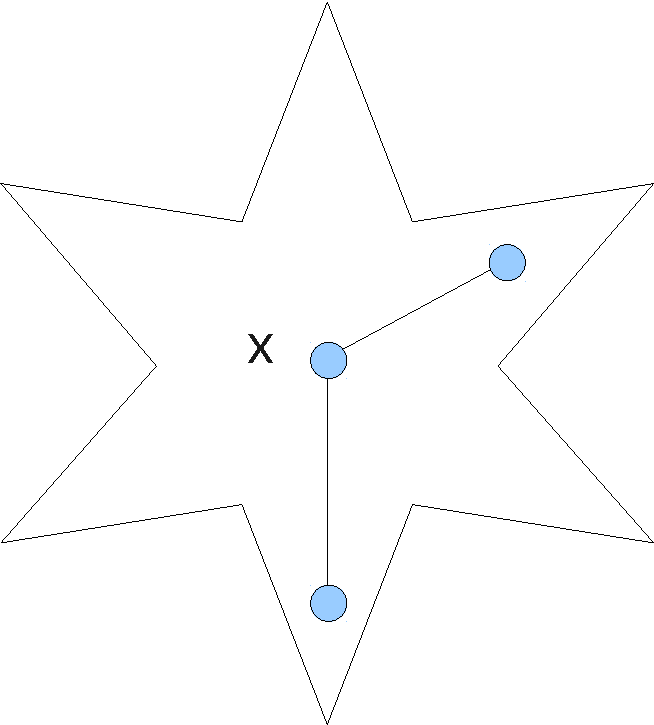
\includegraphics[scale=0.3]{images/ouvert_etoile.pdf}
%\end{center}
%\caption{Ouvert étoilé non convexe}\label{ch8:fig6}
%\end{figure}

Rappelons qu'une $1$-forme est dite \textbf{exacte}, s'il existe une fonction $f$ telle que $\omega=\diff f$ ; et dans ce cas $\diff \omega=\diff^2 f= 0$. Une $1$-forme $\omega$ telle que $\diff \omega =0$ est dite \textbf{fermée} ; un exemple important de forme fermée est $\omega = f \diff z$ avec $f$ holomorphe (\ref{eq:formclosed}). On peut se demander s'il existe une réciproque : étant donnée une $1$-forme fermée, peut-on trouver une fonction $f$ telle que $\omega=\diff f$. Ceci est l'objet du théorème de Poincaré.

\begin{fthm}
Soit $U$ un ouvert étoilé et $\omega$ une $1$-forme fermée sur $U$, alors $\omega$ est exacte, c'est à dire qu'il existe une fonction lisse $f$ sur $U$ telle que $\omega = \diff f$.
\end{fthm}

\begin{proof}
La preuve de ce théorème est intéressante par la façon de construire la fonction $f$ ; une technique qui sera étendue ultérieurement avec la notion de primitive le long d'un chemin. 

\begin{figure}[ht]
\begin{center}
\begin{tikzpicture}[line cap=round,line join=round,>=triangle 45,x=1.0cm,y=1.0cm, scale=0.7]
  \tikzset{
  % style to apply some styles to each segment of a path
  on each segment/.style={
    decorate,
    decoration={
      show path construction,
      moveto code={},
      lineto code={
        \path [#1]
        (\tikzinputsegmentfirst) -- (\tikzinputsegmentlast);
      },
      curveto code={
        \path [#1] (\tikzinputsegmentfirst)
        .. controls
        (\tikzinputsegmentsupporta) and (\tikzinputsegmentsupportb)
        ..
        (\tikzinputsegmentlast);
      },
      closepath code={
        \path [#1]
        (\tikzinputsegmentfirst) -- (\tikzinputsegmentlast);
      },
    },
  },
  % style to add an arrow in the middle of a path
  mid arrow/.style={postaction={decorate,decoration={
        markings,
        mark=at position .5 with {\arrow[#1]{stealth}}
      }}},
}   
\clip(-2,-5) rectangle (13,6);
\fill[line width=1.2pt,color=black,fill=pblue,fill opacity=0.05000000074505806] (6.06,5.82) -- (4.,3.) -- (1.04,3.3) -- (2.66,1.) -- (0.94,-1.68) -- (3.84,-1.6) -- (6.,-4.36) -- (8.02,-1.64) -- (11.06,-1.8) -- (9.,1.) -- (11.08,3.26) -- (8.,3.) -- cycle;
\draw [line width=1.2pt,color=black] (6.06,5.82)-- (4.,3.);
\draw [line width=1.2pt,color=black] (4.,3.)-- (1.04,3.3);
\draw [line width=1.2pt,color=black] (1.04,3.3)-- (2.66,1.);
\draw [line width=1.2pt,color=black] (2.66,1.)-- (0.94,-1.68);
\draw [line width=1.2pt,color=black] (0.94,-1.68)-- (3.84,-1.6);
\draw [line width=1.2pt,color=black] (3.84,-1.6)-- (6.,-4.36);
\draw [line width=1.2pt,color=black] (6.,-4.36)-- (8.02,-1.64);
\draw [line width=1.2pt,color=black] (8.02,-1.64)-- (11.06,-1.8);
\draw [line width=1.2pt,color=black] (11.06,-1.8)-- (9.,1.);
\draw [line width=1.2pt,color=black] (9.,1.)-- (11.08,3.26);
\draw [line width=1.2pt,color=black] (11.08,3.26)-- (8.,3.);
\draw [line width=1.2pt,color=black] (8.,3.)-- (6.06,5.82);
\draw [line width=1.2pt,postaction={on each segment={mid arrow=red}}] (5.4,0.36)-- (6.24,2.38);
\draw [line width=1.2pt,postaction={on each segment={mid arrow=red}}] (6.24,2.38)-- (7.46,2.38);
\draw [line width=1.2pt,postaction={on each segment={mid arrow=red}}] (5.4,0.36)-- (7.46,2.38);
\begin{scriptsize}
\draw [fill=pblue] (5.4,0.36) circle (2.5pt);
\draw[color=black] (5.,0.2) node {{\normalsize $P$}};
%\draw[color=black] (5.2,1.5) node {{\normalsize $\gamma$}};
\draw [fill=pblue] (6.24,2.38) circle (2.5pt);
\draw[color=black] (5.8,2.5) node {{\normalsize $Q$}};
\draw [fill=pblue] (7.46,2.38) circle (2.5pt);
\draw[color=black] (8.6,2.5) node {{\normalsize $Q + h e_1$}};
\end{scriptsize}
\end{tikzpicture}
\caption{Illustration pour la preuve du théorème de Poincaré.}\label{fig:Poincare}
\end{center}
\end{figure}


Soit $P \in U$, un point par rapport auquel $U$ est étoilé. On souhaite construire une fonction $f$ en tout point $Q \in U$. Pour cela, nous considérons le segment $\gamma(t)=P + t v$, avec $v=(Q-P)$ et $t \in [0,1]$, qui par hypothèse a son image inclus dans $U$. On peut ainsi définir $f(Q)$ en intégrant la forme différentielle $\omega = \alpha \diff x + \beta \diff y$ sur ce chemin :
\[f(Q) = \int_\gamma \omega=\int_{[0,1]} \omega_{\gamma(t)}\cdot v \diff t.\]

Nous allons montrer que $\partial_x f=\alpha$ et $\partial_y f=\beta$. Pour cela, considérons l'expression 
\[ \frac{f(Q+ h e_1)-f(Q)}{h},\]
lorsque $h$ tend vers $0$. Soit $\gamma_1$, le segment reliant les points $P$ et $Q + h e_1$ ($e_1,e_2$ sont les vecteurs de base de $\mathbb{R}^2$) (cf. figure~\ref{fig:Poincare}), alors $\gamma_1(t) = P + t(v + h e_1)$, $t \in [0,1]$. Alors 
\[\frac{f(Q+ h e_1)-f(Q)}{h}  = \frac{1}{h} \left( \int_{\gamma_1} \omega  - \int_{\gamma} \omega \right)=I_1 + I_2\]
avec si $v = v_x e_1 + v_y e_2$~:
\begin{align*}
I_1 & =\int_{[0,1]} \Bigl[ \frac{1}{h} \bigl( \alpha(P + t v + t h e_1) - \alpha(P + t v) \bigr) v_x + \alpha(P + t v + t h e_1)\Bigr] \diff t \\
I_2 & = \int_{[0,1]} \Bigl[ \frac{1}{h} \left( \beta(P + tv + t h e_1) - \beta(P + t v) \right) v_y \Bigr] \diff t
\end{align*}
Pour $h \rightarrow 0$ et en appliquant le théorème de dérivation sous le signe somme 
on obtient:
\[\lim_{h \rightarrow 0} \frac{f(Q+ h e_1)-f(Q)}{h} = \int_{[0,1]}  \Bigl[ t \Bigl(\partial_x
\alpha(P+tv) v_x  +  \partial_x
\beta(P+tv)v_y \Bigr)+ \alpha(P+tv) \Bigr]  \diff t.\]
Par hypothèse $\diff \omega = 0$, donc $\partial_x \beta=\partial _y \alpha$
et l'expression précédente devient:
\begin{align*}
\partial_x f (Q) & =  \int_{[0,1]}  \Bigl[ t \Bigl(\partial_x
\alpha(P+tv) v_x  +  \partial_y
\alpha(P+tv)v_y \Bigr)+ \alpha(P+tv) \Bigr]  \diff t \\
&= \int_{[0,1]}  \Bigl[ t  \frac{\diff}{\diff t} \alpha(P + t v)+ \alpha(P+tv) \Bigr]  \diff t.
\end{align*}
Par intégration par parties, nous obtenons finalement
\[\partial_x f (Q) = \left[t \alpha(p+tv)\right]_0^1 = \alpha(Q),
\]
prouvant bien que $\partial_x f = \alpha$ pour tous les points $Q \in U$. On montrerait de même que $\partial_y f = \beta$, ce qui termine la preuve. En fait, nous avons également prouver que $\int_{\gamma_1 -\gamma} \omega=\int_{\sigma} \omega$ où $\sigma$ est le segment horizontal reliant $Q$ à $Q + h e_1$. Ce qui peut se formuler que l'intégrale de $\omega$ sur le lacet $\gamma + \sigma-\gamma_1$ est nulle ; nous y reviendrons dans la suite. 
\end{proof}
Il est intéressant de noter que si l'hypothèse $\diff \omega =0$ n'est pas vérifiée,
on peut néanmoins construire $f$ et bien sûr calculer $\diff f$ comme dans la preuve
précédente. Le terme résiduel qui dans ce cas rend différentes les formes $\diff f$
et $\omega$ peut d'exprimer, avec quelques manipulations simples, uniquement en
fonction de $\diff \omega$, donnant en quelque sorte une généralisation du théorème.

La formule de Stokes, qui dans le cas de $\mathbb{R}^2$ porte aussi le nom de
théorème de Green-Riemann, est essentiellement une formule d'intégration par
parties pour les formes différentielles. Elle permet de transformer une
intégrale sur un ouvert de $\mathbb{R}^2$ en une intégrale sur son bord, au même
titre que la formule d'intégration par parties transforme une intégrale sur un
intervalle en une différence entre des valeurs prises sur ses extrémités.
La preuve de cette formule remarquable est délicate, nous l'énoncerons sans démonstration, pour plus de détails se reporter à \cite{cartan1977}, par exemple.  

%\begin{fprop}
%Soit $U$ un ouvert de $\mathbb{R}^2$, $\Phi \colon V \to U$ un difféomorphisme
%de classe $C^{k+1}$ et $\omega=\alpha dx + \beta dy$ une forme différentielle de
%classe $C^k$ et de degré $1$ sur $U$. Soit enfin $\gamma$ un chemin de classe $C^1$ par morceaux
%dont l'image est contenue dans $V$. On a:
%\[
%\int_{\Phi \circ \gamma} \omega = \int_{\gamma} \Phi^*\omega
%\]
%\end{fprop}
%
%\begin{proof}
%On notera encore $\Phi = \phi e_1 + \psi e_2$. 
%Par définition:
%\begin{align*}
%\int_{\Phi \circ \gamma} \omega = & \int_{[0,1]}
%\alpha\left((\Phi\circ\gamma)(t)\right) \frac{d}{dt}(\phi(\gamma(t))) \\
%& + \beta\left((\Phi\circ\gamma)(t)\right) \frac{d}{dt}(\psi(\gamma(t))) dt
%\end{align*}
%Le théorème des fonctions composées donne, en notant $\gamma^\prime_x,
%\gamma^\prime_y$ les composantes de $\gamma^\prime$ selon $e_1,e_2$:
%\[
%\frac{d}{dt}(\phi(\gamma(t))) = \frac{\partial \phi}{\partial
%x}\gamma^\prime_x(t) + \frac{\partial \phi}{\partial
%y}\gamma^\prime_y(t)
%\]
%et de même:
%\[
%\frac{d}{dt}(\psi(\gamma(t))) = \frac{\partial \psi}{\partial
%x}\gamma^\prime_x(t) + \frac{\partial \psi}{\partial
%y}\gamma^\prime_y(t)
%\]
%En regroupant les termes dans l'intégrale, on obtient:
%\begin{align*}
%& \int_{\Phi \circ \gamma} \omega = \\ &\int_{[0,1]}
%\left(\alpha\left((\Phi\circ\gamma\right)(t)\frac{\partial \phi}{\partial
%x}(t) +\beta\left((\Phi\circ\gamma\right)(t)\frac{\partial \psi}{\partial
%x}(t)  + \right)\gamma^\prime_x(t) \\
%& + \left(\alpha\left((\Phi\circ\gamma\right)(t)\frac{\partial \phi}{\partial
%y}(t) +\beta\left((\Phi\circ\gamma\right)(t)\frac{\partial \psi}{\partial
%y}(t)  + \right)\gamma^\prime_y(t) dt = \\
%& \int_{\gamma} \Phi^*\omega
%\end{align*}
%\end{proof}
%
%\begin{fprop}{(Théorème de Stokes élémentaire)}
%Soit $\omega=\alpha dx + \beta dy$ une forme différentielle de classe $C^1$
%définie sur un ouvert $U$ de $\mathbb{R}^2$, nulle en dehors d'un compact $K
%\subset U$. On a:
%\[
%\int_{H^+} d \omega = \int_{\mathbb{R}} \alpha(x,0)dx
%\]
%Avec $H^+ = \mathbb{R} \times \mathbb{R}^+$ le demi-espace formé des points de
%$\mathbb{R}^2$ à ordonnée positive.
%\end{fprop}
%
%\begin{proof}
%La situation est résumée sur la figure \ref{ch8:fig7}. La preuve repose sur le
%théorème de Fubini, et est élémentaire dans ce cas. On a par définition:
%\[
%d \omega = \left( \frac{- \partial \alpha }{\partial y} + \frac{\partial
%\beta}{\partial x} \right) dx dy
%\] 
%et:
%\[
%\int_{H^+} d\omega = \int_{\mathbb{R}\times \mathbb{R}^+}  \left(-
%\frac{\partial \alpha }{\partial y} + \frac{\partial \beta}{\partial x} \right) dxdy
%\]
%Le théorème de Fubini s'applique et on a:
%\[
%\int_{\mathbb{R}\times \mathbb{R}^+}-\frac{ \partial \alpha }{\partial
%y}(x,y)dxdy = \int_{\mathbb{R}} \left(\int_{\mathbb{R}^+} -\frac{\partial \alpha
%}{\partial y}(x,y)dy \right) dx
%\]
%Comme $\alpha$ est à support compact:
%\[
%\int_{\mathbb{R}^+} -\frac{\partial \alpha }{\partial
%y}(x,y)dy = \alpha(x,0)
%\]
%De même par Fubini:
%\[
%\int_{\mathbb{R}\times \mathbb{R}^+}\frac{\partial \beta }{\partial
%x}(x,y)dxdy = \int_{\mathbb{R}^+} \left(\int_{\mathbb{R}} \frac{\partial
%\beta }{\partial x}(x,y)dx \right) dy
%\]
%Par compacité du support de $\beta$:
%\[
%\int_{\mathbb{R}} \frac{\partial
%\beta }{\partial x}(x,y)dx = 0
%\]
%qui donne le résultat demandé.
% \begin{figure}[ht]
%\begin{center}
%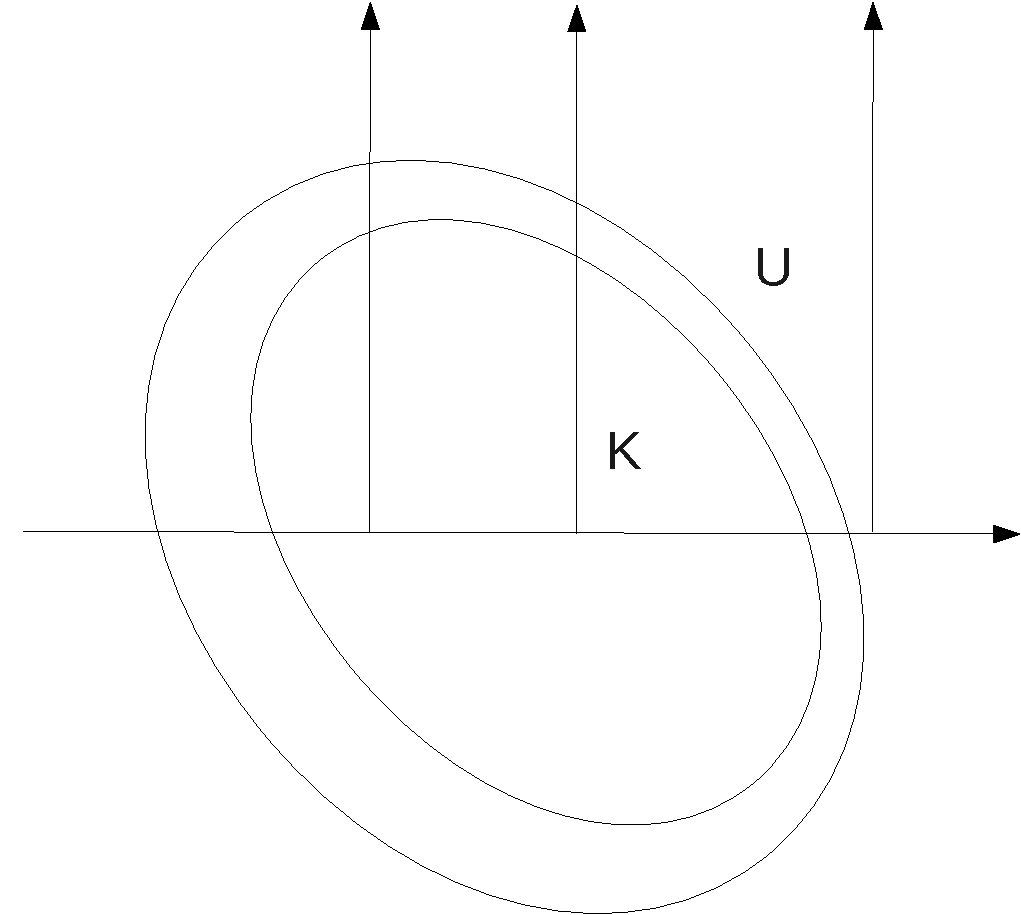
\includegraphics[scale=0.3]{images/stokes_elem.pdf}
%\end{center}
%\caption{Intégration de $d\omega$ par Fubini}\label{ch8:fig7}
%\end{figure}
%\end{proof}
%On remarquera l'intégrale sur $\mathbb{R}^+$ peut être vue comme une intégrale de
%chemin, en considérant pour cela un chemin correspondant à un segment de l'axe
%réel et contenant le support de $\omega$.
%On notera également que si le support de $\alpha$ a une intersection vide avec
%l'axe réel positif, l'intégrale est nulle. Le cas général du théorème de Stokes
%va s'obtenir en recollant des morceaux sur lesquels on le résultat élémentaire
%pourra s'appliquer. La proposition suivante donne un procédé permettant un
%découpage très régulier et s'utilise assez couramment.
%\begin{fdefn}
%On dira qu'un recouvrement ouvert $(U_i)_{i \in I}$ d'une partie $A \subset
%\mathbb{R}^n$ est localement fini si tout point $x \in A$ possède un voisinage
%ne rencontrant qu'un nombre fini d'ouverts du recouvrement.
%\end{fdefn}
% \begin{fprop}{(Partitions de l'unité)}
% Soit $(U_i)_{i \in I}$ un recouvrement ouvert localement fini d'un ouvert $U
% \subset \mathbb{R}^n$. Il existe une famille d'applications $(\xi_i)_{j \in J}$ à
% valeurs dans $[0,1]$ telle que~:
% \begin{itemize}
%   \item $\forall j \in J \exists i \in I \, supp(\xi_j) \subset U_i$.
%   \item $\sum_{j \in J} \xi_j = 1$, où $1$ désigne l'application constante
%   égale à 1.
% \end{itemize}
% \end{fprop}
%La famille obtenue par la proposition précédente s'appelle partition de l'unité
%subordonnée au recouvrement $(U_i)_{i \in I}$. La somme intervenant dans la
%proposition est algébrique~: pour tout $x \in U$, il ne peut exister qu'un
%nombre fini d'indices $j$ tels que $\xi_j(x) \neq 0$. Ceci apparaîtra clairement
%au cours de la démonstration.
%\begin{proof}
%On remarquera tout d'abord qu'il existe une famille croissante de compacts
%(pour la topologie induite sur $U$) $(K_n)_{n \in \mathbb{N}}$ telle que
%$\cup_{n \in \mathbb{N}} K_n = U$ et $K_n \subset \overset{\circ}{K_{n+1}}$. Il suffit pour cela de prendre $K_n =
%U \cap \overline{B(0,n)}$. Pour $n$ fixé, l'ensemble
%$\tilde{K}_n = K_{n+1} - \overset{\circ}{K_{n}}$ est un compact car fermé
%dans le compact $K_{n+1}$. On peut recouvrir $\tilde{K_n}$ par les ouverts
%$O_{n,i} =  (\overset{\circ}{K}_{n+2} - K_{n-1}) \cap U_i$.Pour tout $x \in
%O_{n,i}$, il est possible de trouver une boule ouverte $B(x,3r_x) \subset
%O_{n,i}$. Soit $\psi \colon [0,1] \to [0,1]$ une application $C^\infty$ telle
%que $\psi(0)=0, \psi(1)=1$ (voir le chapitre sur la transformation de Fourier
%pour l'existence d'une telle fonction).
%On définit $\theta_x$ par:
%\[
%\theta \colon y \mapsto \left \{
%\begin{array}{cc}
%1 & \text{ si } y \in B(x,r_x) \\
%0 & \text{ si } y \in B(x,3r_x) - B(x,2r_x) \\
%\psi\left(2 - \frac{\|y-x\|}{r_x}\right) & \text{ si } y \in B(x,2r_x) -
%B(x,r_x)
%\end{array}
%\right .
%\]
% Les boules ouvertes $B(x,r_x)$ forment un recouvrement ouvert du compact $\tilde{K}_n$, 
% on peut donc en extraire un sous-recouvrement fini déterminé par les points $x_{j,n}, i \in J_n$. 
% La collection $B(x_{j,n}, r_{x_{j,n}}), n \in
%\mathbb{N}, j \in  J_n$ est dénombrable et vérifie les propriétés suivantes~:
%\begin{itemize}
%  \item Pour tout couple d'indices ${j,n}$, il existe $i \in I$ tel que
%  $supp(\theta_{x_{j,n}}) \subset U_i$.
%  \item Pour tout point $x \in U$, il n'existe qu'un nombre fini d'observables
%  de la famille $\theta_{x_{j,n}}$ ne s'annulant pas en $x$.
%  \item Pour tout point $x \in U$, il existe au moins une fonction
%  de la famille $\theta_{x_{j,n}}$ ne s'annulant pas en $x$. 
%\end{itemize}
%Pour terminer la démonstration on pose~:
%\[
%\xi_{k,l} = \frac{\theta_{x_{k,l}}}{\sum_{n,j\in J_n} \theta_{x_{j,n}}} 
%\]
%\end{proof}

\begin{fthm}{(Théorème de Stokes)}
Soit $U$ un ouvert de $\mathbb{R}^2$ dont le bord $\partial U$ est un \textbf{lacet simple}
de classe $C^1$ par morceaux, parcouru dans le sens trigonométrique. Soit $\omega$ une $1$-forme différentielle
définie sur $U$ et continue sur $U \cup  \partial U$. On a : 
\[
\int_{U} \diff \omega = \int_{\partial U} \omega.
\]
\end{fthm}

%\begin{proof}
%On ne donne ici qu'une idée de la preuve. Le lecteur pourra essayer de l'écrire
%complètement. On supposera qu'en tout point $t$
%de l'intervalle $[0,1]$, $\gamma^\prime(t) \neq 0$. En application du théorème d'inversion locale, on peut
%trouver, pour tout point de $\gamma(t)$, un voisinage ouvert  $V$ de ce point et
%un difféomorphisme $\Phi$ de classe $C^1$ sur un ouvert $W$ tel que
%$\Phi(U\cap V) \in W\cap H^+$ et $\Phi(\gamma([0,1])\cap V)$ soit dans
%l'intersection de $W$ avec l'axe réel. On peut imposer de plus
%que $\Phi(\gamma(t))$ décrive un segment de l'axe réel d'abscisse croissante
%avec $t$. L'image de $\gamma$ étant compacte, on peut extraire de la famille
%précédente un sous-recouvrement fini. En y ajoutant l'ouvert $U$ lui-m\^eme, 
%on peut construire une partition de l'unité subordonnée à cette famille. 
%Sur la partie correspondant à $U$, l'intégrale de $d\omega$ est nulle.
% Sur les autres morceaux, on peut appliquer Stokes élémentaire: 
% les intégrales de chemin étant invariantes par difféomorphisme, on en déduit le
%résultat.
%\end{proof}

%\begin{rem} La formule de Stokes illustre le lien entre la différentielle extérieure et l'opérateur \og bord \fg{} $\partial$ d'un ouvert, puisque si nous notons l'intégration par un crochet de dualité $\langle \cdot, \cdot \rangle$, nous obtenons pour tout ouvert $U$ à bord un lacet simple et toute $1$-forme, l'identité
% \[\langle U, \diff \omega \rangle = \langle \partial U, \omega \rangle.\]
%\end{rem}

\begin{rem}
La condition de continuité de la forme sur $U \cup \partial U$ a pour but d'écarter les comportements exotiques sur la frontières des coefficients de la forme. Il est possible de s'en passer en se restreignant à l'intégration sur tout compact $K$ inclus dans $U$ (cf. \cite{cartan1977}).
\end{rem}

Une conséquence fondamentale du théorème de Stokes est que l'intégrale d'une
$1$-forme fermée sur un lacet simple est nulle.

\begin{exem}
Soit la $1$-forme $\omega=-y \diff x + x \diff y$, alors $\diff \omega = 2 \diff x \wedge \diff y$. Pour tout lacet simple $\gamma$, considéré comme le bord d'un domaine ouvert $U$, nous avons
\[\int_\gamma \omega = \int_U \diff \omega = 2 \int_U \diff x \diff y = 2 \text{aire}(U).\]
Ainsi, si $U$ est le disque unité, $\gamma$ étant alors le cercle de rayon $1$, nous obtenons $\int_\gamma \omega =2 \pi$.

Notons qu'en notation complexe la forme $\bar{z}\diff z$ s'écrit comme la somme $\omega_1 + i \omega$, où $\omega_1=x \diff x + y \diff y$ est une forme fermée, d'où
\[\int _\gamma \bar{z} \diff z=  i  2 \, \text{aire}(U).\]
\end{exem}

\section{Exercices complémentaires}

\begin{exer}
Exprimer $\diff \lvert z \rvert$ en termes de $\diff z$ et $\diff \bar{z}$.
\end{exer}

\begin{exer}
Soit la $1$-forme $\omega=(1/z) \diff z$ définie sur le disque ouvert unité privé de l'origine. 
\begin{MYenumerate}
\item Exprimer $\omega$ sous la forme $\omega = \omega_1 + i \omega_2$ où $\omega_1$ et $\omega_2$ sont des $1$-formes à coefficients des fonctions réelles.
\item Montrer que $\omega_1$ et $\omega_2$ sont fermées.
\item Montrer que $\omega_1$ est exacte sur l'ouvert $\{ 0<\lvert z \rvert <1\}$ en trouvant $f_1$ telle que $\omega_1=\diff f_1$
\item Montrer que $\omega_2$ est exacte sur le demi-plan de droite $\{ (x,y) : x>0\}$ (\textsc{indication :} considérer la fonction $f_2(x,y)=\arctan(y/x)$. 
\item Que représente l'intégrale de $\omega_2$ pour un chemin inclus dans le demi-plan de droite (cf. figure~\ref{fig:exer3_2})?
\item Expliquer pourquoi cette forme n'est pas exacte dans $\{ 0<\lvert z \rvert <1\}$. 
 \end{MYenumerate}
\begin{figure}[H]
\begin{center}
\shorthandoff{!}\shorthandoff{:}
\begin{tikzpicture}
\tikzset{
    on each segment/.style={
        decorate,
        decoration={
            show path construction,
            moveto code={},
            lineto code={
                \path [#1]
                (\tikzinputsegmentfirst) -- (\tikzinputsegmentlast);
            },
            curveto code={
                \path [#1] (\tikzinputsegmentfirst)
                .. controls
                (\tikzinputsegmentsupporta) and (\tikzinputsegmentsupportb)
                ..
                (\tikzinputsegmentlast);
            },
            closepath code={
                \path [#1]
                (\tikzinputsegmentfirst) -- (\tikzinputsegmentlast);
            },
        },
    },
}
%\draw[->] (-1,0) -- (5,0);
%\draw (5,0) node[right] {$x$};
\draw [->] (0,0) -- (0,5);
\draw (0,5) node[above] {$y$}; 
\draw[fill=black] (0,2) circle (2pt);
    \begin{scope}[scale=2, xshift=1.cm, yshift=0.5cm, rotate=70]
        \node (A) at (0,0) {};
        \node (B) at (2,0.25){};
        \draw[blue] plot [smooth,tension=1]
        coordinates {(A) (1,0) (1.14,-0.6) (0.5,-0.5) (0.5,0.5) (1.5,0) (B)}[postaction={on each segment={draw,-{stealth[red,bend]}}}];
%  %      \draw (1, -1) node {chemin quelconque};
        \draw [fill=black] (A) circle (1pt);
    \draw [fill=black] (B) circle (1pt);
    \end{scope}

%\node (A) at (1,0.5) {};
% \node (B) at (2,4.25){};
%\draw [fill=black] (A) circle (2pt);
%\draw [fill=black] (B) circle (2pt);
%\draw[blue] plot [smooth,tension=1]
%coordinates {(A) (1,0) (2.14,-0.6) (1.5,-0.5) (0.5,0.5) (1.5,0) (B)}[postaction={on each segment={draw,-{stealth[red,bend]}}}];
\draw (0,2) -- (A);
\draw (0,2) -- (B);       
\end{tikzpicture}
\shorthandon{!}\shorthandoff{:}
\end{center}
\caption{} \label{fig:exer3_2}
\end{figure}
\end{exer}


\begin{exer}[Lemme 1.14 dans \cite{fulton1997algebraic}]
Soit $U_1, U_2$ deux ouverts de $\R^2$ tels que $U_1 \cap U_2$ soit connexe. Soit $U=U_1 \cup U_2$ et soit $\omega$ une $1$-forme sur $U$. 
\begin{MYenumerate}
\item Montrer que si les restrictions de $\omega$ à $U_1$ et $U_2$ sont respectivement exactes, alors $\omega$ est exacte sur $U$ (\textsc{Indication :} Poser $\omega=\diff f_1$ sur $U_1$ et $\omega=\diff f_2$ sur $U_2$, et considérer la différentielle de la fonction $(f_2-f_1)$ sur $U_1\cap U_2$ connexe).
\item Montrer l'importance de l'hypothèse de connexité de l'intersection en considérant la forme différentielle $\omega_2$ sur le disque unité privé du centre, introduite dans l'exercice précédent (\textsc{indication :} prendre pour $U_1$ (resp. $U_2$) le demi-plan de droite (resp. de gauche) avec des extensions au-delà de l'axe $x=0$, sans contenir l'origine de sorte et noter que l'intersection $U_1 \cap U_2$ n'est pas connexe cf. figure~\ref{fig:exer3_3}).
\end{MYenumerate}

\begin{figure}[H]
\begin{center}
\shorthandoff{!}\shorthandoff{:}
\begin{tikzpicture}[line cap=round,line join=round,>=triangle 45,x=1.0cm,y=1.0cm, scale=0.5]
\tikzset{
    on each segment/.style={
        decorate,
        decoration={
            show path construction,
            moveto code={},
            lineto code={
                \path [#1]
                (\tikzinputsegmentfirst) -- (\tikzinputsegmentlast);
            },
            curveto code={
                \path [#1] (\tikzinputsegmentfirst)
                .. controls
                (\tikzinputsegmentsupporta) and (\tikzinputsegmentsupportb)
                ..
                (\tikzinputsegmentlast);
            },
            closepath code={
                \path [#1]
                (\tikzinputsegmentfirst) -- (\tikzinputsegmentlast);
            },
        },
    },
}
%\draw [color=black, xstep=1.0cm,ystep=1.0cm] (-4.3,-11.6) grid (29.78,6.3);
%\draw[->,color=black] (-4.3,0.) -- (29.78,0.);
%\foreach \x in {-4.,-3.,-2.,-1.,1.,2.,3.,4.,5.,6.,7.,8.,9.,10.,11.,12.,13.,14.,15.,16.,17.,18.,19.,20.,21.,22.,23.,24.,25.,26.,27.,28.,29.}
%\draw[shift={(\x,0)},color=black] (0pt,2pt) -- (0pt,-2pt) node[below] {\footnotesize $\x$};
%\draw[->,color=black] (0.,-11.6) -- (0.,6.3);
%\foreach \y in {-11.,-10.,-9.,-8.,-7.,-6.,-5.,-4.,-3.,-2.,-1.,1.,2.,3.,4.,5.,6.}
%\draw[shift={(0,\y)},color=black] (2pt,0pt) -- (-2pt,0pt) node[left] {\footnotesize $\y$};
%\draw[color=black] (0pt,-10pt) node[right] {\footnotesize $0$};
\clip(0,-5) rectangle (15,6.3);
\fill[line width=1pt,color=black,fill=gray!30] (3.,4.) -- (12.,4.) -- (12.,-3.) -- (8.,-3.) -- (8.,2.) -- (3.,2.) -- cycle;
\fill[line width=1.2pt,color=green,fill=gray!30] (6.,3.) -- (1.,3.) -- (1.,-4.) -- (11.,-4.) -- (11.,0.) -- (6.,0.) -- cycle;
\draw [line width=0.5pt] (3.,4.)-- (12.,4.);
\draw [line width=0.5pt] (12.,4.)-- (12.,-3.);
\draw [line width=0.5pt] (12.,-3.)-- (8.,-3.);
\draw [line width=0.5pt] (8.,-3.)-- (8.,2.);
\draw [line width=0.5pt] (8.,2.)-- (3.,2.);
\draw [line width=0.5pt] (3.,2.)-- (3.,4.);
\draw [line width=0.5pt] (6.,3.)-- (1.,3.);
\draw [line width=0.5pt] (1.,3.)-- (1.,-4.);
\draw [line width=0.5pt] (1.,-4.)-- (11.,-4.);
\draw [line width=0.5pt] (11.,-4.)-- (11.,0.);
\draw [line width=0.5pt] (11.,0.)-- (6.,0.);
\draw [line width=1pt] (6.,0.)-- (6.,3.);
\fill[line width=0.pt,color=red,fill=red,pattern=north east lines,pattern color=black] (3.,3.) -- (6.,3.) -- (6.,2.) -- (3.,2.) -- cycle;
\fill[line width=0.pt,color=red,fill=red,pattern=north east lines,pattern color=black] (8.,0.) -- (11.,0.) -- (11.,-3.) -- (8.,-3.) -- cycle;
\draw[fill=black] (7,1) circle (2pt);
\draw (7,1) node[right]{$0$} ;
\draw (10,2) node[right]{$U_1$} ;
\draw (4,-2.2) node[below]{$U_2$} ;
\draw[blue] plot [smooth]
        coordinates {(3.5,2.5) (2,1) (2.5,-1) (5,-2) (7,-2.4) (10, -2) (10.5, 0) (9.5, 2.2) (7.5,3)  (3.5,2.5)}[postaction={on each segment={draw,-{stealth[red,bend]}}}];
\draw[fill=black] (3.5,2.5) circle (3pt);
\draw (3.5,2.5) node[below]{$A$} ;
\draw[fill=black] (10,-2) circle (3pt);
 \draw (10,-2) node[right]{$B$} ; 
     
\end{tikzpicture}
\end{center}
\caption{} \label{fig:exer3_3}
\end{figure}
\end{exer}

\begin{exer}\label{exer:recollement}
Considérons à nouveau l'exemple illustré en figure~\ref{fig:exer3_3}. Soit $\omega$ une $1$-forme fermée dans $U=U_1 \cup U_2$, et soit $ \gamma$ le lacet entourant l'origine, dont l'image est incluse dans $U$. 
\begin{MYenumerate}
\item En posant $\omega=\diff f_1$ dans $U_1$ et $\omega=\diff f_2$ dans $U_2$, montrer qu'il est possible de choisir $f_1$ et $f_2$ telle que $f_1=f_2$ dans la partie hachurée contenant le point $A$.
\item Calculer l'intégrale de $\omega$ sur le lacet en fonction de la valeur $f_1 -f_2$ sur la partie hachurée contenant le point $B$.
\end{MYenumerate}
\end{exer}




\begin{exer}
Soit $\omega \diff z + q \diff \bar{z} = \alpha \diff x + \beta \diff y$, une $1$-forme sur un ouvert $U$ de $\R^2$. On définit la $1$-forme différentielle
\[\ast \omega = i p\diff z - i q \diff \bar{z} = -\beta \diff x + \alpha \diff y.\]
\begin{MYenumerate}
\item Montrer que $**\omega=-\omega$ et calculer $\diff \ast \omega$ en termes de $\diff z, \diff \bar{z}$ et $\diff x, \diff y$. Appliquer au cas où $\omega$ est exacte : (i.e. calculer $\ast \diff f$, avec $f$ fonction lisse sur $U$.
\item Une $1$-forme $\omega$ est dite harmonique si $\diff \omega=\diff \ast \omega=0$. Donner une condition nécessaire et suffisante pour $\omega$ soit harmonique.
\item Soit $f$ une fonction lisse sur $U$, calculer $\diff (\ast \diff f)$.

\end{MYenumerate}



\end{exer}

\newpage 
\subsection*{Un peu d'histoire \dots}

\begin{minipage}{0.2\linewidth}
\begin{center}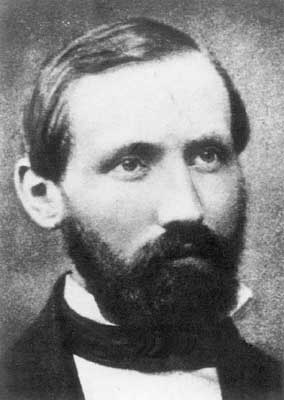
\includegraphics[width=2cm]{images/Riemann.jpg}\end{center}
\end{minipage}
\begin{minipage}{0.80 \linewidth}
\small{\paragraph*{Bernhard Riemann :} né le  17 Septembre 1826 à Breselenz, mort le 20 Juillet 18666 à Semasca (Italie). Riemann est un des mathématiciens les plus importants de son époque et peut être de tous les temps. Durant sa courte carrière, il fonde la géométrie différentielle et contribue puissamment à l'étude des fonctions de la variable complexe. Il formalise la notion d'intégrale à partir de subdivisions de l'intervalle d'intégration.}
\end{minipage}

\vfill

\begin{minipage}{0.2\linewidth}
\begin{center}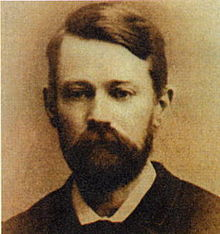
\includegraphics[width=2cm]{images/Stieltjes.jpg}\end{center}
\end{minipage}
\begin{minipage}{0.80\linewidth}
\small{\paragraph*{Thomas Joannes Stieltjes :} né le 29 décembre 1856 à Zwolle (Pays-Bas), mort le 31 décembre 1894 à Toulouse. Il travaillera sur les fractions continues, les formules de quadratures de Gauss et généralisera l'intégrale de Riemann.}
\end{minipage}
\vfill
\begin{minipage}{0.2\linewidth}
\begin{center} 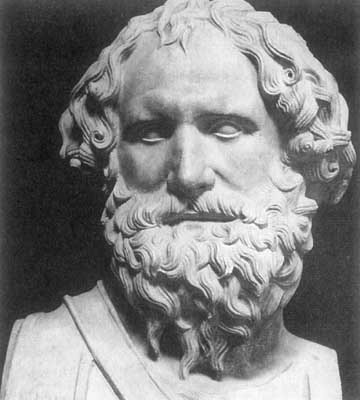
\includegraphics[width=2cm]{images/archimede.jpg} \end{center}
\end{minipage} 
\begin{minipage}{0.80\linewidth}
\small{\paragraph*{Archimède :} né à Syracuse  vers 287 av. J.-C. et mort à Syracuse en 212 av. J.-C. Génie universel, un des plus grands mathématiciens de tous les temps. Précurseur du calcul intégral, il invente la méthode d'approximation des périmètres par les chemins polygonaux. Sa défense du de Syracuse lors de son attaque par la flotte romaine et sa mort de la main d'un soldat sont particulièrement célèbres, ainsi que son exclamation \og Eureka\fg{} (j'ai trouvé). On lui doit aussi l'invention de la vis, de l'écrou  et des roues dentées !}
\end{minipage}
\vfill


\begin{minipage}{0.2\linewidth}
\begin{center}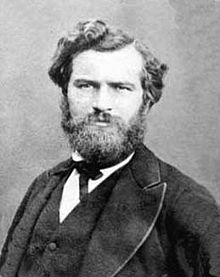
\includegraphics[width=2cm]{images/Jordan.jpg}\end{center}
\end{minipage}
\begin{minipage}{0.80\linewidth}
\small{\paragraph*{Camille Jordan :} né à Lyon le 5 Janvier 1838 et mort à Paris le 22 Janvier 1922. Ingénieur de formation, il enseigne les mathématiques à l'école polytechnique et au collège de France. On lui doit un remarquable cours d'analyse, ainsi que de nombreuses contributions en théorie des groupes.}
\end{minipage}
\vfill

\begin{minipage}{0.2\linewidth}
 \begin{center}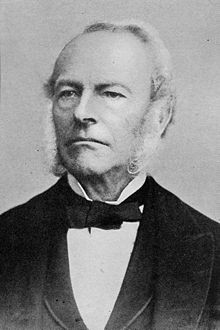
\includegraphics[width=2cm]{images/Stokes.jpg}\end{center}
\end{minipage}
\begin{minipage}{0.80\linewidth}
\small{\paragraph*{George Gabriel Stokes :} né le  	13 août 1819 dans le Comté de Sligo (Irlande), mort le 1er février 1903 à Cambridge (Angleterre). Contribue à l'étude de la mécanique des fluide visqueux. Il explique la fluorescence de certains matériaux. Le théorème sur l'intégration des formes différentielles qui porte son nom est en réalité dû à Lord Kelvin (voir ci-dessous).}
\end{minipage}
\vfill

\begin{minipage}{0.2\linewidth}
\begin{center}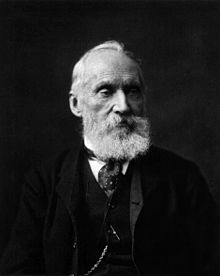
\includegraphics[width=2cm]{images/Kelvin.jpg}\end{center}
\end{minipage}
\begin{minipage}{0.80\linewidth}
\small{\paragraph*{Lord Kelvin :} né le 26 juin 1824 à Belfast, mort le 17 décembre 1907 à
Largs. Physicien britannique très connu pour ses travaux en thermodynamique. On lui doit le second principe de cette science et l'échelle de température qui porte son nom. Il contribue aussi à l'électricité et à la mécanique et est un des pionniers de l'analyse vectorielle. }
\end{minipage}